\section{Additional Related Work}
\label{sec:related-work}

\subsection{Compute Scaling}\label{app:scaling-laws}

\Cref{eq:scaling-law_joint}  omits the hyperparameters, describing loss at the \emph{fully tuned frontier}: the best attainable loss given the parameters and data 
% (Figure~\ref{fig:scaling-laws-at-the-fully-tuned-frontier})
; however, parameters and data do not vary independently. The model's gradients must be computed for every example, so their product determines the total compute: $c \propto p d$.
Given a budget, you face a trade-off between larger models and longer training. Navigating this trade-off is exactly why people turn to scaling laws. Minimizing \Cref{eq:scaling-law_joint} with fixed compute yields the condition:
%
\begin{equation}\label{eq:compute-optimality-condition}
    \iota \frac{\zeta}{p^\iota} = \kappa \frac{\eta}{d^\kappa}
\end{equation}
%
Hence the optimal parameters and data become power laws in compute:
%
\begin{equation}\label{eq:compute-optimal-parameters-and-data}
    p \propto c^{\frac{\kappa}{\iota + \kappa}} \qquad d \propto c^{\frac{\iota}{\iota + \kappa}}
\end{equation}
%
If you plug these values into the joint scaling law then you obtain excess loss as a power law in the compute:
%
\begin{equation}\label{eq:scaling-law_compute}
    \mathcal{L}(p, d) - \epsilon \propto c^{-\frac{\iota\kappa}{\iota + \kappa}}
\end{equation}
%
Thus scaling laws reveal the best loss given the compute and how to get it by balancing parameters and data.

\citet{Hoffmann2022AnEmpirical} found balanced parameters and data grow at the same rate, a conclusion since echoed by many others \citep{anil2023palm2technicalreport, deepseekai2024deepseekllmscalingopensource}. This idea justifies the token-to-parameter ratio as a meaningful measure of how well-trained a model is, with the compute-optimal ratio serving as baseline. Under \Cref{eq:compute-optimality-condition}, this same-rate growth only occurs when the scaling exponents are equal: $\iota = \kappa$. Some theoretical work predicts this equality \citep{Bahri2024Explaining}, and the estimates are often close in practice. Researchers have also explored enforcing it to improve estimation \citep{Muennighoff2025Scaling, li2025misfitting}.


\subsection{The Noisy Quadratic Limit}
\label{app:background:the-noisy-quadratic-limit}

How do we know if the hyperparameters are fully tuned, or how hard that is to accomplish? The \emph{noisy quadratic limit} answers these questions. \citet{lourie2025hyperparameter} found that near the optima, loss surfaces are:
%
\begin{enumerate}[noitemsep]
    \item \textbf{Quadratic}: well approximated by the second-order Taylor expansion;
    \item \textbf{Low-Rank}: governed by a few directions that explain most of the variation; and
    \item \textbf{Normal}: distributed about the mean as additive normal noise.
\end{enumerate}
%
Empirically, this approximation holds for a large region around the optimum, the \emph{asymptotic regime}. This region determines the practical questions we care about, like tuning difficulty or the best attainable performance.

Formally, if $\bX$ are the hyperparameters, $Y$ the validation score, and $(\bx_*, y_*)$ the optimum, then the conditional distribution $Y\mid\bX$ is approximately a quadratic plus additive normal noise, $E$.\footnote{
    Integral hyperparameters (e.g., batch size) can be treated as continuous; discrete ones are handled with separate quadratics.
} Letting $H_{\bx_*}$ be the Hessian:
%
\begin{equation}\label{eq:noisy-quadratic-structure}
    \mathcal{L}(\bX) \approx y_* + \left(\bX - \bx_*\right)^T H_{\bx_*} \left(\bX - \bx_*\right) + E, \qquad E \sim \normal(0, \sigma)
\end{equation}

This conditional view induces a marginal structure that emerges during random search. More precisely, the search induces a distribution over validation scores, and that distribution's tail converges to a \textit{noisy quadratic distribution}, $\quadratic_{\min}(\alpha, \beta, \gamma, \sigma)$. Writing $F(y; \alpha, \beta, \gamma, \sigma)$ for the CDF of the noisy quadratic distribution, then:
%
\begin{equation}\label{eq:noisy-quadratic-limit}
    \Prob(Y \leq y) \approx F(y; \alpha, \beta, \gamma, \sigma) \quad\text{ as }\quad y \to y_*.
\end{equation}
%
The distribution's parameters capture properties of the loss surface: $\alpha$ is the best attainable performance ($y_*$), $\beta$ measures how tightly the scores concentrate around it, $\gamma$ gives the \textit{effective} number of hyperparameters (intrinsic dimension at the optimum), and $\sigma$ represents the noise due to random seeds. In practice, we define the asymptotic regime by a threshold on the expected loss, $\E[Y\mid\bX] \leq \theta$, marking where this structure holds.


The \textbf{noisy quadratic distribution} arises as the sum $Q + E$, where $Q \sim \quadratic_{\min}(\alpha, \beta, \gamma)$ is the (noiseless) quadratic distribution and $E \sim \normal(0, \sigma)$ is independent Gaussian noise. The noiseless quadratic is supported on $[\alpha, \beta]$ with CDF and density
%
\begin{equation}\label{eq:quadratic-cdf}
    F_Q(y; \alpha, \beta, \gamma) = \left(\frac{y - \alpha}{\beta - \alpha}\right)^{\gamma/2},
    \qquad
    f_Q(y; \alpha, \beta, \gamma) = \frac{\gamma}{2(\beta - \alpha)}\left(\frac{y - \alpha}{\beta - \alpha}\right)^{\frac{\gamma - 2}{2}},
\end{equation}
%
for $\alpha \leq y \leq \beta$ (and $0$, resp. $1$, outside). Its lower tail decays polynomially with exponent $\gamma/2$, encoding the ellipsoidal volume of near-optimal hyperparameters: the rank of the Hessian sets $\gamma$, so higher intrinsic dimension makes near-optimal configurations rarer. Convolving with the Gaussian gives the noisy quadratic, supported on all of $\reals$, with CDF and density
%
\begin{align}\label{eq:noisy-quadratic-cdf}
    F(y; \alpha, \beta, \gamma, \sigma)
        &= \Phi\!\left(\frac{y - \beta}{\sigma}\right)
            + \int_{0}^{1} v^{\gamma/2}\, p_V(v)\, \d v,
    \\ \label{eq:noisy-quadratic-pdf}
    f(y; \alpha, \beta, \gamma, \sigma)
        &= \frac{\gamma}{2(\beta - \alpha)} \int_{0}^{1} v^{\frac{\gamma - 2}{2}}\, p_V(v)\, \d v,
\end{align}
%
where $\Phi$ is the standard normal CDF and $p_V$ is the density of $V \sim \normal\!\left(\frac{y - \alpha}{\beta - \alpha}, \frac{\sigma}{\beta - \alpha}\right)$. 
The $\Phi$ term accounts for noise carrying scores past $\beta$, while the truncated integral convolves the quadratic tail with the noise over the support $[\alpha, \beta]$ (i.e., $v \in [0, 1]$). 
As $\sigma \to 0$, the integral concentrates and \Cref{eq:noisy-quadratic-cdf} recovers the noiseless quadratic \Cref{eq:quadratic-cdf}. 



\subsection{Downstream Scaling laws}
\label{sec:appendix-Downstream-Scaling-laws}

\begin{wrapfigure}{r}{0.7\textwidth}
    \centering
    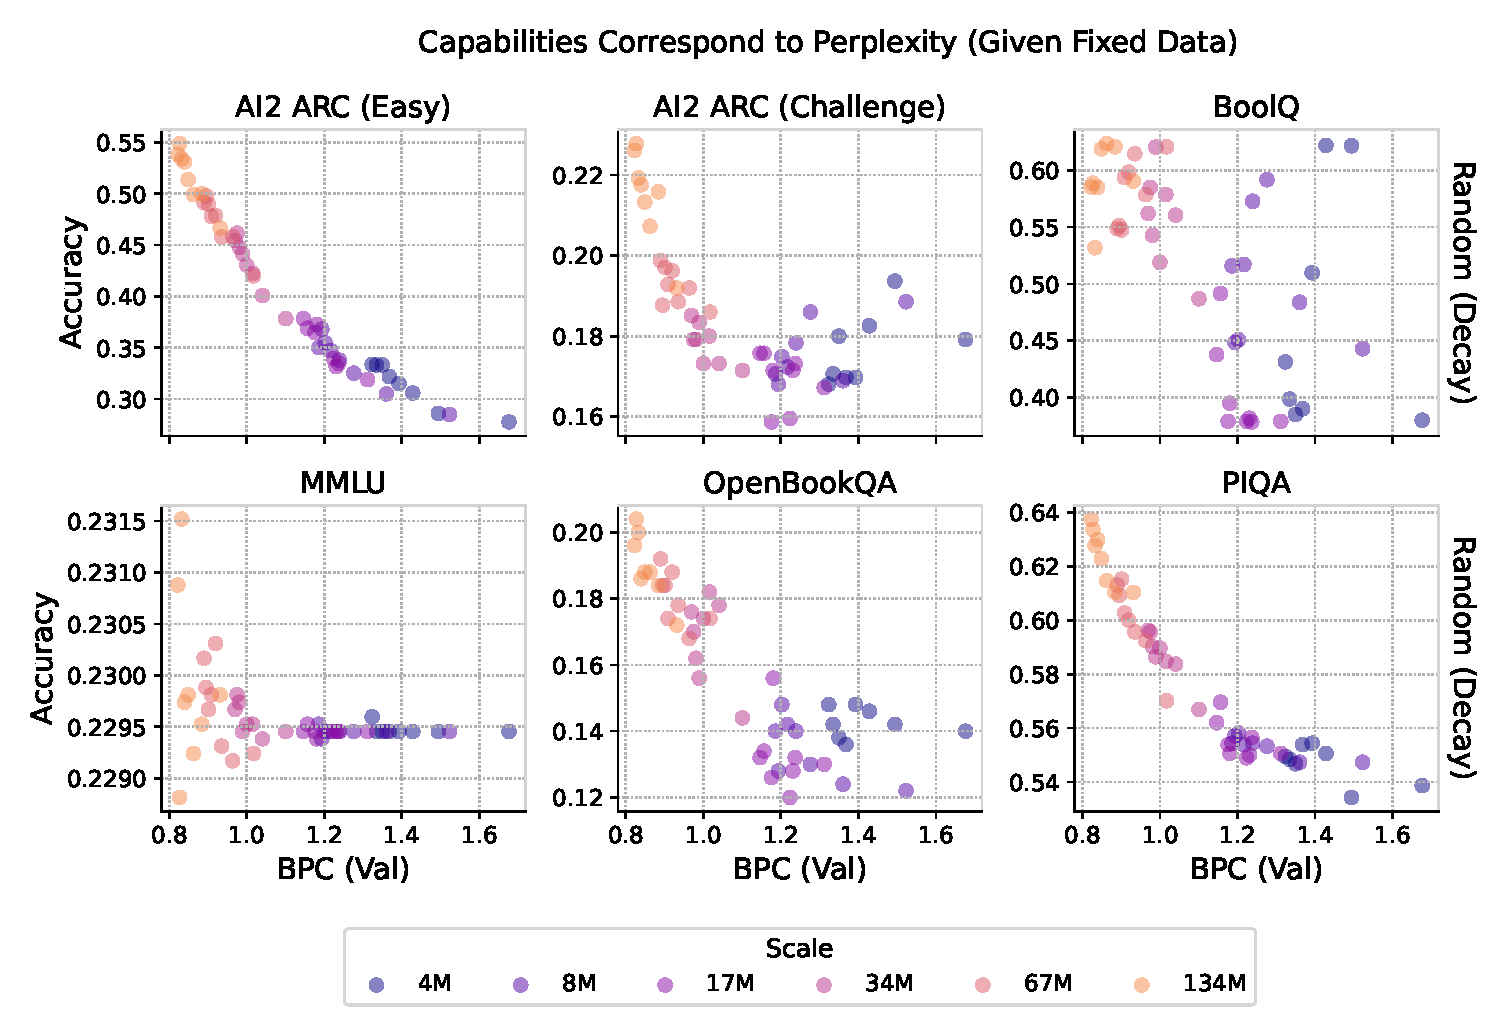
\includegraphics[width=0.95\linewidth]{figures/perplexity-corresponds-to-capabilities.pdf}
    \caption{
        \emph{Given a fixed corpus, perplexity corresponds to downstream capability across a wide variety of tasks.} The relationship between pretraining loss and capability is not always predictable or even monotonic; however, models achieving the same loss have a similar conditional distribution over their capabilities as we increase parameters and data, or even randomize the architecture, as long as the \emph{composition} of pretraining data remains fixed.
    }
    \label{fig:perplexity-corresponds-to-capabilities}
\end{wrapfigure}



The data defines a curve of capabilities; the loss decides a point on that curve; the scaling law determines the cost of that point. \Cref{fig:perplexity-corresponds-to-capabilities} illustrates this principle: models trained at different scales or for different lengths fall along a single (possibly noisy) curve. The curve varies wildly across tasks, but exists for all of them. Regardless of whether better capabilities lie down the road, the scaling law sets the toll. In other words a model with a better scaling law achieves every perplexity, and thus any capability, at lower cost.





